\documentclass[uplatex,dvipdfmx,a4paper,js=standard, titlepage]{bxjsarticle}
\usepackage[dvipdfmx]{graphicx}
\usepackage{h31ec-exp}
\makeatletter
\newcommand{\figcaption}[1]{\def\@captype{figure}\caption{#1}}
\newcommand{\tblcaption}[1]{\def\@captype{table}\caption{#1}}
\makeatother

\title{半導体素子の静特性の測定}
\grade{3年32番}
\author{平田 蓮}
\team{第B班}
\date{2019年6月24日}
\expdate{2019年6月10日,6月17日,6月24日}
\coauthor{
    2番 & 朝倉 大智 \\
    12番 & 小室 弦太 \\
    22番 & 髙野 新士
 }

\begin{document}
\maketitle
\section{実験A ダイオードとツェナダイオードの静特性}
    \subsection{目的}
        \begin{itemize}
            \item pn接合半導体素子(ダイオード)の順方向, ~逆方向の電圧-電流特性を測定する.
            \item 逆方向の電圧を増加させた時に,
                ~ある電圧になると電流が急増する降伏特性を利用したツェナダイオードの電圧-電流特性を測定する.
            \item 交流入力に対する半波整流特性を観測することにより,
                ~ダイオードの整流特性について学習する.
        \end{itemize}
    \subsection{実験方法}
        \subsubsection{注意点}
            \begin{itemize}
                \item 電源のスイッチをONにする前に, ~回路の接続と計測機器の設定を十分に確認する.
                \item 各実験について, ~電圧や電流の範囲が指定された値を超えないよう,
                    ~注意しながら実験を進める.
                \item 電圧や電流の測定値は表にまとめ, ~電圧-電流の関係をグラフにまとめる.
                \item 観察波形は考察で困らないように, ~概形を記録し, ~必要な数値, ~条件をメモしておく.
            \end{itemize}
        \subsubsection{ダイオードの特性}
            図\ref{fig:diode_forward}, ~\ref{fig:diode_reverse}にダイオード特性測定用回路を示す.
            \begin{figure}[ht]
                \begin{minipage}{0.5\hsize}
                    \begin{center}
                        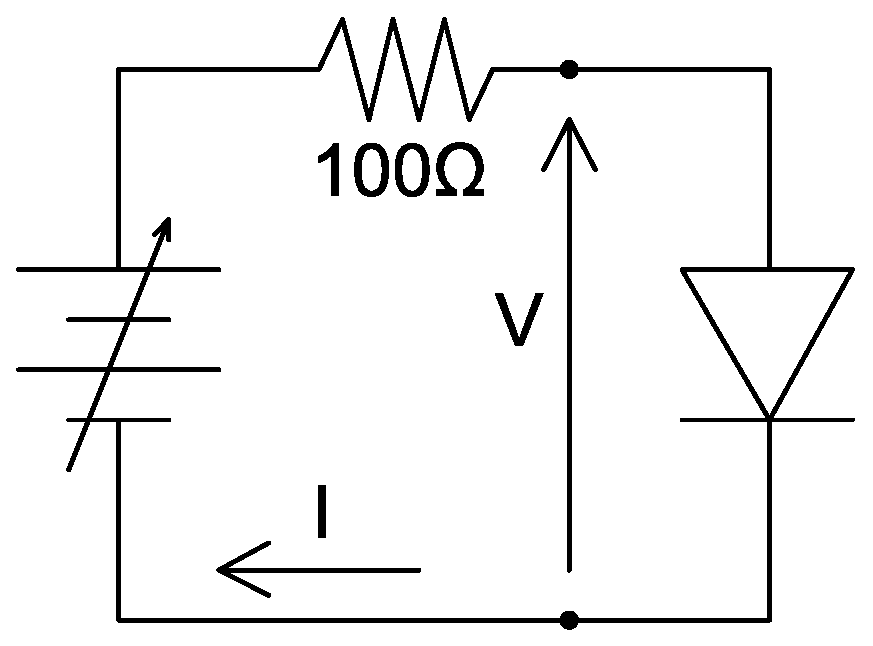
\includegraphics[width=6cm]{images/diode_forward.eps}
                        \caption{ダイオード順方向特性測定回路}
                        \label{fig:diode_forward}
                    \end{center}
                \end{minipage}
                \begin{minipage}{0.5\hsize}
                    \begin{center}
                        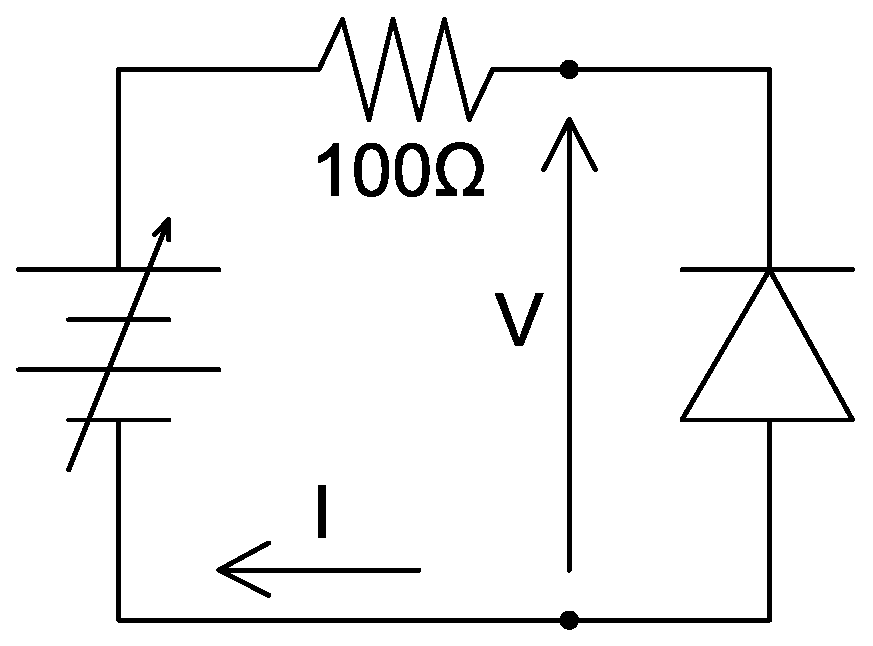
\includegraphics[width=6cm]{images/diode_reverse.eps}
                        \caption{ダイオード逆方向特性測定回路}
                        \label{fig:diode_reverse}
                    \end{center}
                \end{minipage}
            \end{figure}

            順方向特性は, ~ダイオードに印加する電圧を変化させ, ~電圧-電流特性を測定する.
            ~この時, ~順方向電流が50[mA]を超えないようにする.

            逆方向特性は, ~ダイオードに印加する電圧を0〜5[V]の範囲で変化させ, ~電圧-電流特性を測定する.
        \subsubsection{ツェナダイオードの特性}
            図\ref{fig:zener_reverse}, \ref{fig:zener_forward}にツェナダイオードの特性測定用回路を示す.
            \begin{figure}[ht]
                \begin{minipage}{0.5\hsize}
                    \begin{center}
                        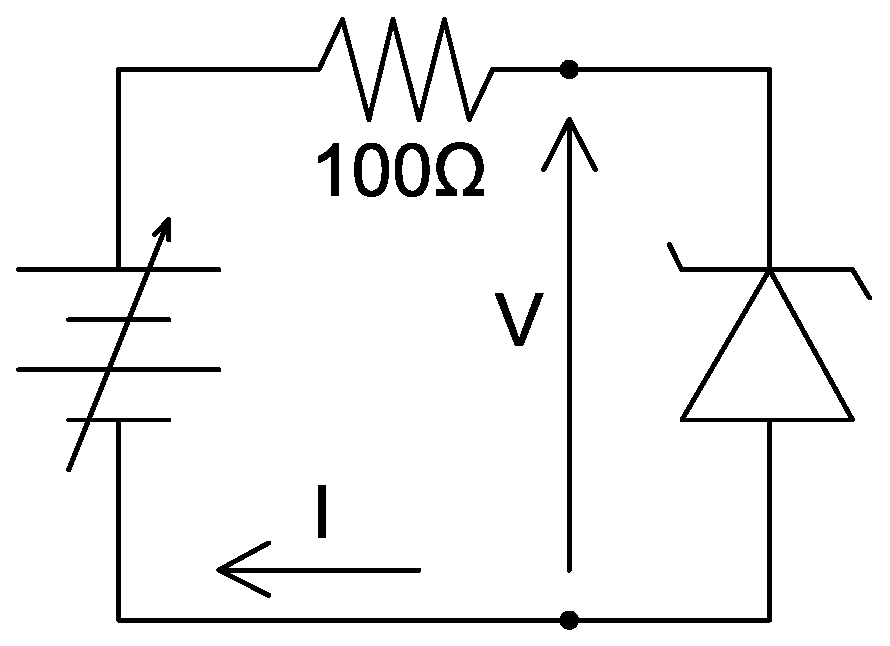
\includegraphics[width=6cm]{images/zener_reverse.eps}
                        \caption{ツェナダイオード逆方向特性測定回路}
                        \label{fig:zener_reverse}
                    \end{center}
                \end{minipage}
                \begin{minipage}{0.5\hsize}
                    \begin{center}
                        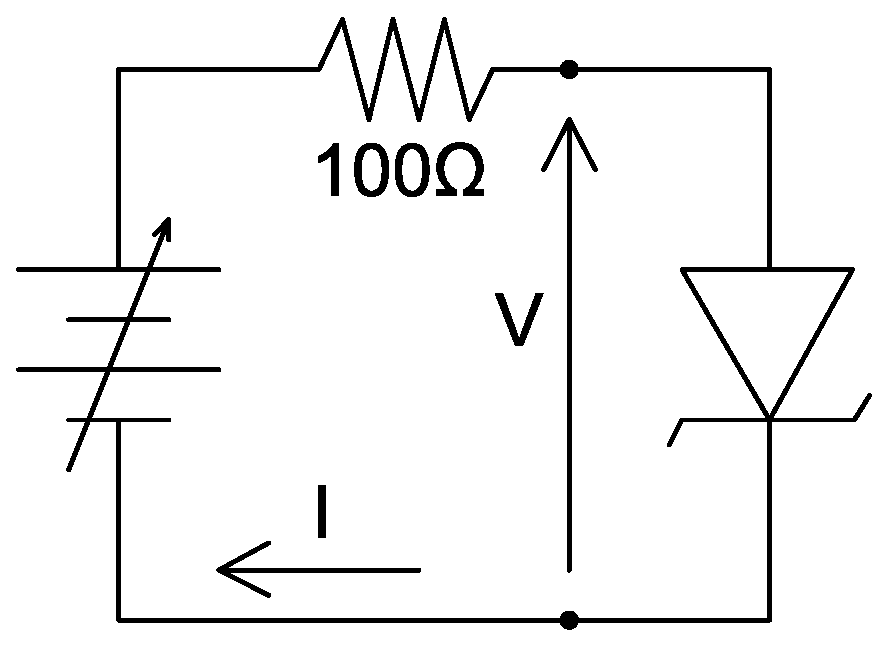
\includegraphics[width=6cm]{images/zener_forward.eps}
                        \caption{ツェナダイオード順方向特性測定回路}
                        \label{fig:zener_forward}
                    \end{center}
                \end{minipage}
            \end{figure}

            ツェナダイオードに印加する電圧を変化させ, ~電圧-電流特性を測定する.
            ~この時, ~順方向, ~逆方向電流が50[mA]を超えないようにする.
        \subsubsection{ダイオードの半波整流特性}
            半波整流回路の図を以下に示す.

            \begin{figure}[ht]
                \begin{center}
                    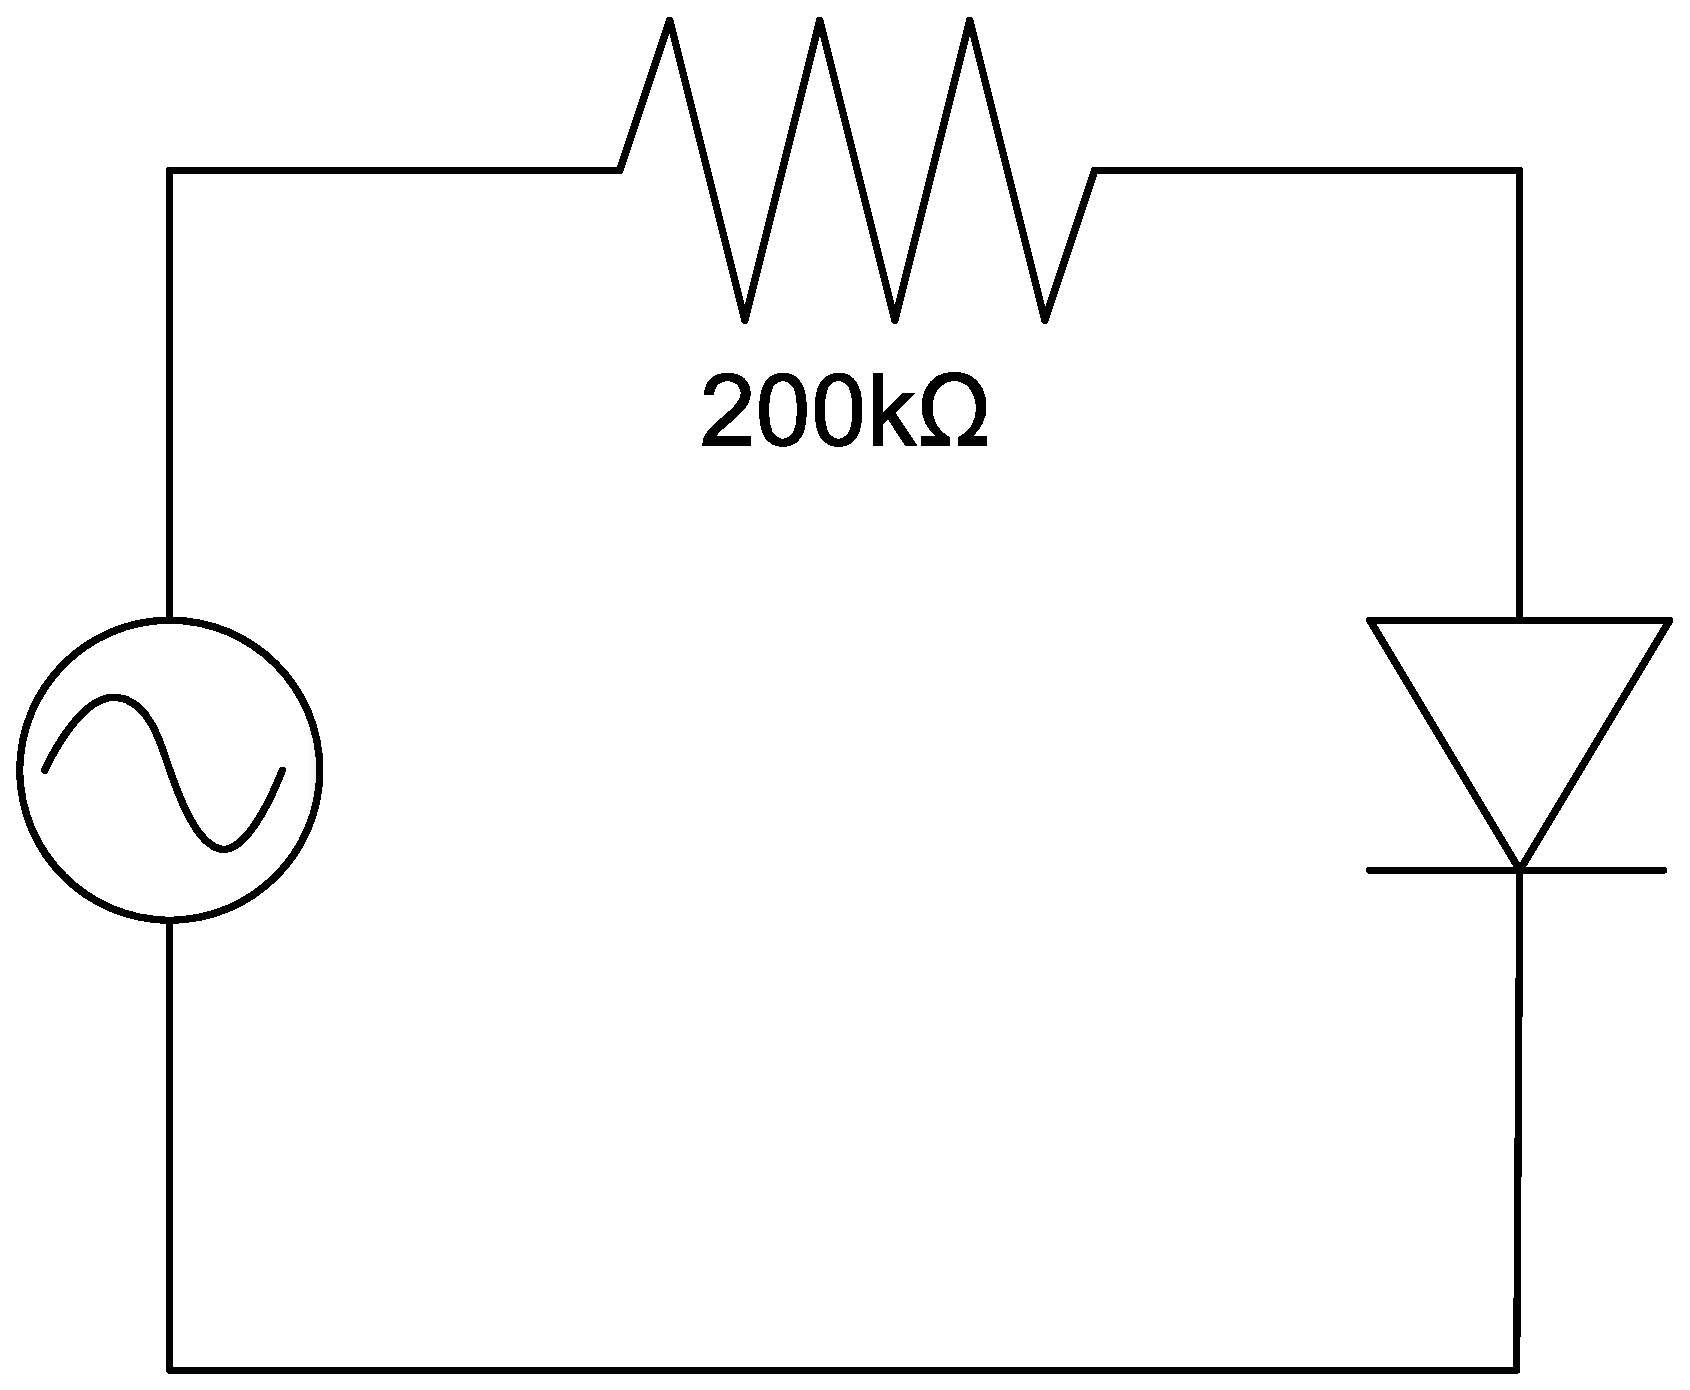
\includegraphics[width=8cm]{images/rectificate.eps}
                    \caption{半波整流回路}
                \end{center}
            \end{figure}

            オシロスコープのCh1で交流電源電圧, ~Ch2で200[k$\Omega$]の両端の電圧を計測できるようにプローブを接続する.
            ~ただし, ~DCモードで測定する. ~また, ~プローブのアースを接続する場所に注意する.

            周波数100[Hz]の正弦波を入力し, ~振幅を0〜6[V]に変えながら次の点について調べる.
            \begin{enumerate}
                \item Ch2の波形が変化し始めた時の正弦波の振幅.
                \item 正弦波の振幅が5[V]の時, ~Ch1とCh2の波形. ~また, ~Ch1とCh2の波形の最大値の差はどのくらいか.
            \end{enumerate}
    \subsection{使用器具}
        \begin{description}
            \item[オシロスコープ] No.20
            \item[ダイオード] EC-02
            \item[デジタルマルチメーター] Ec-17
            \item[直流電源] Ec-09
            \item[交流電源] Ec-05
        \end{description}
    \subsection{実験結果}
        各実験の結果の表とグラフを以下に示す.
        \subsubsection{ダイオードの特性}
            図\ref{fig:diode_graph}, \ref{tab:diode_table}にダイオードの特性のグラフと表を示す.
            ~ここで, ~逆方向電圧の値を負数として表現する.
            \begin{figure}[ht]
                \begin{minipage}{0.5\hsize}
                    \begin{center}
                        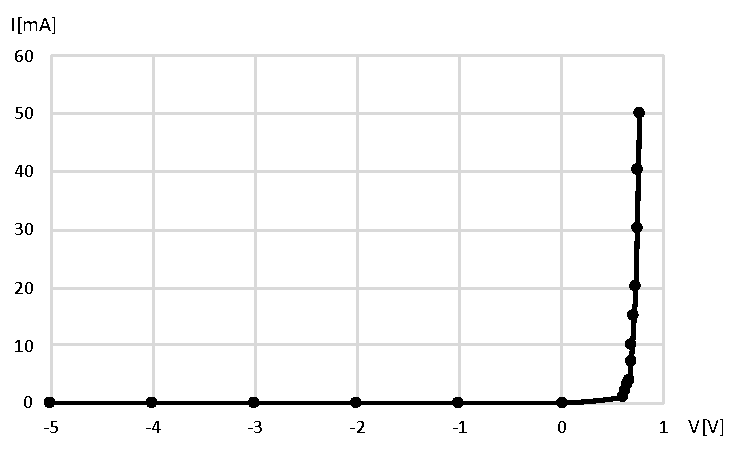
\includegraphics[width=8cm]{graphs/diode_graph.pdf}
                        \caption{ダイオード特性グラフ}
                        \label{fig:diode_graph}
                    \end{center}
                \end{minipage}
                \def\@captype{table}
                \begin{minipage}{0.5\hsize}
                    \begin{center}
                        \caption{ダイオード特性}
                        \label{tab:diode_table}
                        \begin{tabular}{c|c||c|c}
                            $V$[V] & $I$[mA] & $V$[V] & $I$[mA] \\ \hline \hline
                            -5.00 & 0.0 & 0.661 & 4.0 \\
                            -4.00 & 0.0 & 0.678 & 7.0 \\
                            -3.00 & 0.0 & 0.691 & 10 \\
                            -2.00 & 0.0 & 0.708 & 15 \\
                            -1.00 & 0.0 & 0.724 & 20 \\
                            0.00 & 0.0 & 0.738 & 30 \\
                            0.598 & 1.0 & 0.749 & 40 \\
                            0.627 & 2.0 & 0.760 & 50 \\
                            0.642 & 3.0 & \\
                        \end{tabular}
                    \end{center}
                \end{minipage}
            \end{figure}

            このグラフと表を見ると, ~順方向電圧が0.6[V]を超えたあたりから順方向電流が流れてることがわかる.
            ~そして, ~電流は急に増え, ~0.76[V]付近で50[mA]まで達している.

            一方逆方向は, ~いくら電圧をかけても逆方向電流は流れていない.

            この, ~電流が一方向にしか流れない特性を整流性という.
            ~これは, ~ダイオードのpn接合面で, ~拡散により空乏層ができ,
            ~それによりp型半導体内では電子が過剰になり, ~n型内では電子が不足し,
            ~p$\to$nの方向に内部電界が発生するためである.
            ~順方向電圧は内部電界を打ち消すため, ~電流が流れ, ~逆方向電圧は内部電界を強めるので,
            ~電流が流れない.
        \subsubsection{ツェナダイオードの特性}
            図\ref{fig:zener_graph}, \ref{tab:zener_table}にツェナダイオードの特性の結果のグラフと表を示す.
            ~ここで, ~逆方向電圧の値を負数として表現する.
            \begin{figure}[ht]
                \begin{minipage}{0.5\hsize}
                    \begin{center}
                        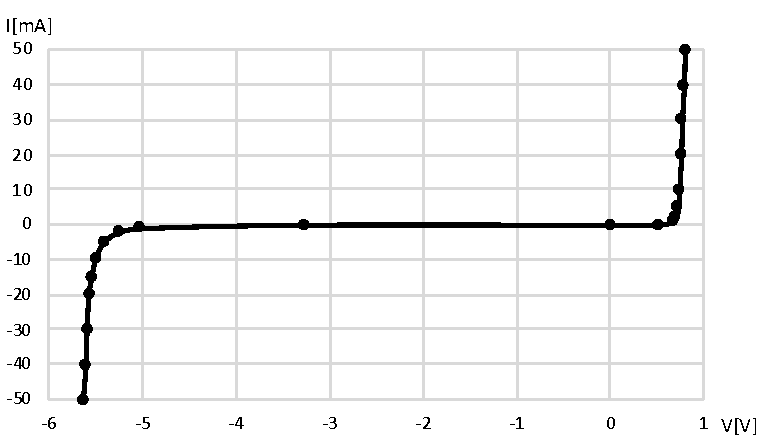
\includegraphics[width=8cm]{graphs/zener_graph.pdf}
                        \caption{ツェナダイオード特性グラフ}
                        \label{fig:zener_graph}
                    \end{center}
                \end{minipage}
                \def\@captype{table}
                \begin{minipage}{0.5\hsize}
                    \begin{center}
                        \caption{ツェナダイオード特性}
                        \label{tab:zener_table}
                        \begin{tabular}{c|c||c|c}
                            $V$[V] & $I$[mA] & $V$[V] & $I$[mA] \\ \hline \hline
                            -5.63 & -50 & -0.00 & 0.0 \\
                            -5.60 & -40 & 0.512 & 0.0 \\
                            -5.59 & -30 & 0.675 & 1.0 \\
                            -5.57 & -20 & 0.694 & 2.0 \\
                            -5.54 & -15 & 0.720 & 5.0 \\
                            -5.50 & -10 & 0.730 & 10 \\
                            -5.41 & -5.0 & 0.750 & 20 \\
                            -5.24 & -2.0 & 0.760 & 30 \\
                            -5.02 & -1.0 & 0.780 & 40 \\
                            -3.28 & 0.0 & 0.790 & 50 \\
                        \end{tabular}
                    \end{center}
                \end{minipage}
            \end{figure}

            グラフと表から, ~順方向はダイオードとほとんど同様に, ~約0.6[V]の電圧をかけた時から順方向電流が流れ始め,
            ~0.79[V]の電圧に達した時に電流が50[mA]に達していることがわかる.

            一方逆方向は, 電圧が5[V]に達したあたりから急激に逆方向電流が流れ始め, 5.6[V]あたりで逆方向電流が50[mA]に達している.

            逆方向電圧が一定を超えると急激に電流が流れ出す現象を降伏現象といい, ~これは高い電圧を加えた際に,
            ~キャリアが半導体内の原子と衝突し, ~さらなるキャリアを生み出すことで起こる.
            ~そのため, ~図のような, ~逆方向にも急激に電流が流れる波形が観察される.

        \subsubsection{ダイオードの半波整流特性}
            図\ref{fig:5[V]の観測波形}, \ref{fig:観測波形の拡大図}に正弦波が5[V]の時の波形の様子とその拡大図を示す.
            ~上の波形がCh1で, ~下がCh2である.
            \begin{figure}[ht]
                \begin{minipage}{0.5\hsize}
                    \begin{center}
                        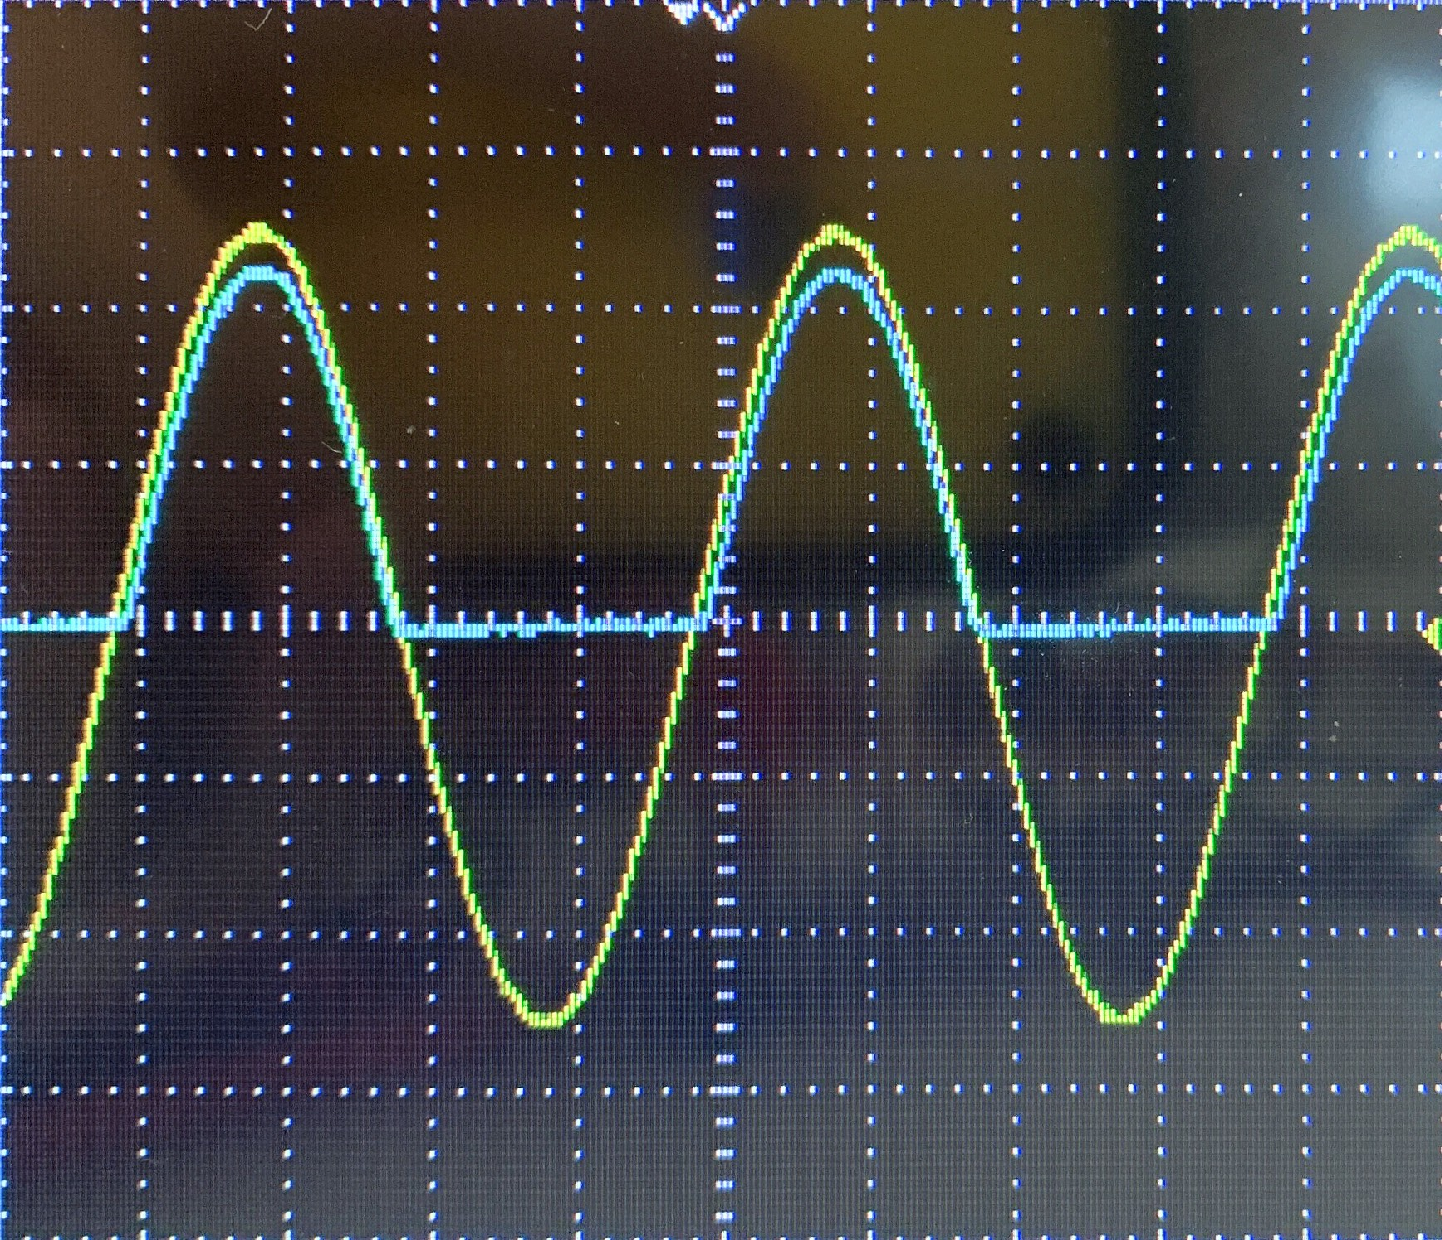
\includegraphics[width=8cm]{images/oscilloscope1.png}
                        \caption{観測波形(振幅5[V]のとき)}
                        \label{fig:5[V]の観測波形}
                    \end{center}
                \end{minipage}
                \begin{minipage}{0.5\hsize}
                    \begin{center}
                        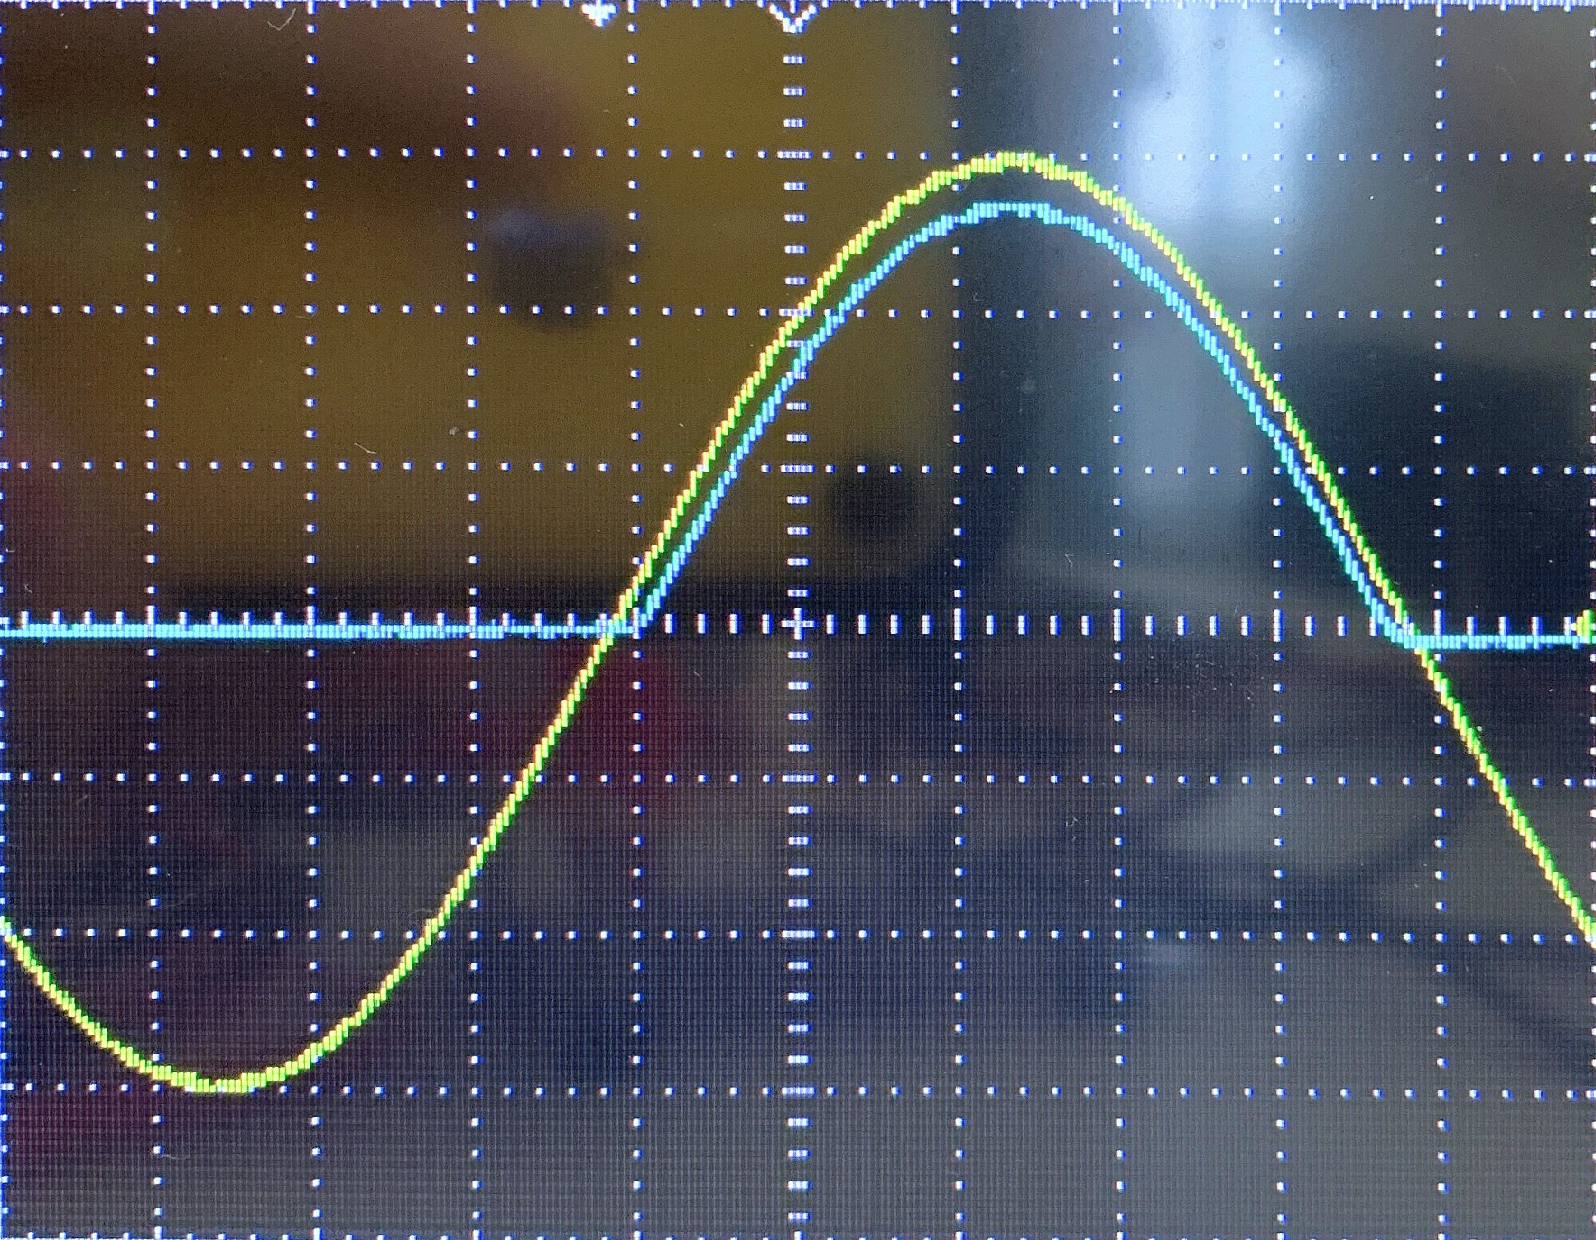
\includegraphics[width=8cm]{images/oscilloscope2.png}
                        \caption{観測波形(拡大図)}
                        \label{fig:観測波形の拡大図}
                    \end{center}
                \end{minipage}
            \end{figure}

            Ch2の波形が変化し始めた時, ~Ch1の振幅は約0.5[V]だった.
            ~この, ~Ch2の波形が変化し始める時のCh1の振幅は,
            ~ダイオードが電流を流し始める時の電圧と同じなので,
            ~Ch2の波形に変化が現れる電圧はダイオードにかかる電圧で決定されると考えられる.

            ~また, ~図の時, ~二つの波形の最大値の差も同様に約0.5[V]だった.
            ~これも, ~上と同様に, ~ダイオードにかかる電圧によって二つの波形に差が生まれていると考えられる.

            ~観察波形の拡大図をよく見ると, ~時間軸の方向にも少し差があることがわかる.
            ~ここには, ~上で述べたことから,
            ~ダイオードに電流が流れる最低限の電圧がかかるまでの時間差が現れていると考えられる.
    \subsection{考察}
        \subsubsection{ツェナダイオードの用途}
            ツェナダイオードは, ~定電圧ダイオードとして使うことができる.
            ~逆方向電圧が一定値を超えると, ~電流が流れ,
            ~電圧がそれ以上上がらなくなるので, ~定電圧をかけることができる.
        \subsubsection{LEDの発光原理}
            ダイオードの中にあるpn結合中で, ~電子とホールが結合する際に,
            ~余分なエネルギーが発生し, ~光として放出される.
            ~これが, ~目で見ることのできるLEDの光である.

            ~また, ~半導体を構成する原子を変えることで, ~光の色を変えることができる.
        \subsubsection{振幅制限器について}
            図\ref{fig:limitter}に示す回路は, ~リミッタ, ~および振幅制限器と呼ばれるものである.
            ~a-b間に電圧がかかると, ~二つのダイオードのどちらかに順方向電圧としてかかる.
            ~電圧が一定値を超え, ~ダイオードに電流が流れ出すと,
            ~ダイオード特性の項で示したようにそれ以上電圧が上がりづらくなる.

            ~よってc-d間には振幅が制限された図\ref{fig:limitter_graph}のような波形が出力されると考えられる.

            \begin{figure}[ht]
                \begin{minipage}{0.5\hsize}
                    \begin{center}
                        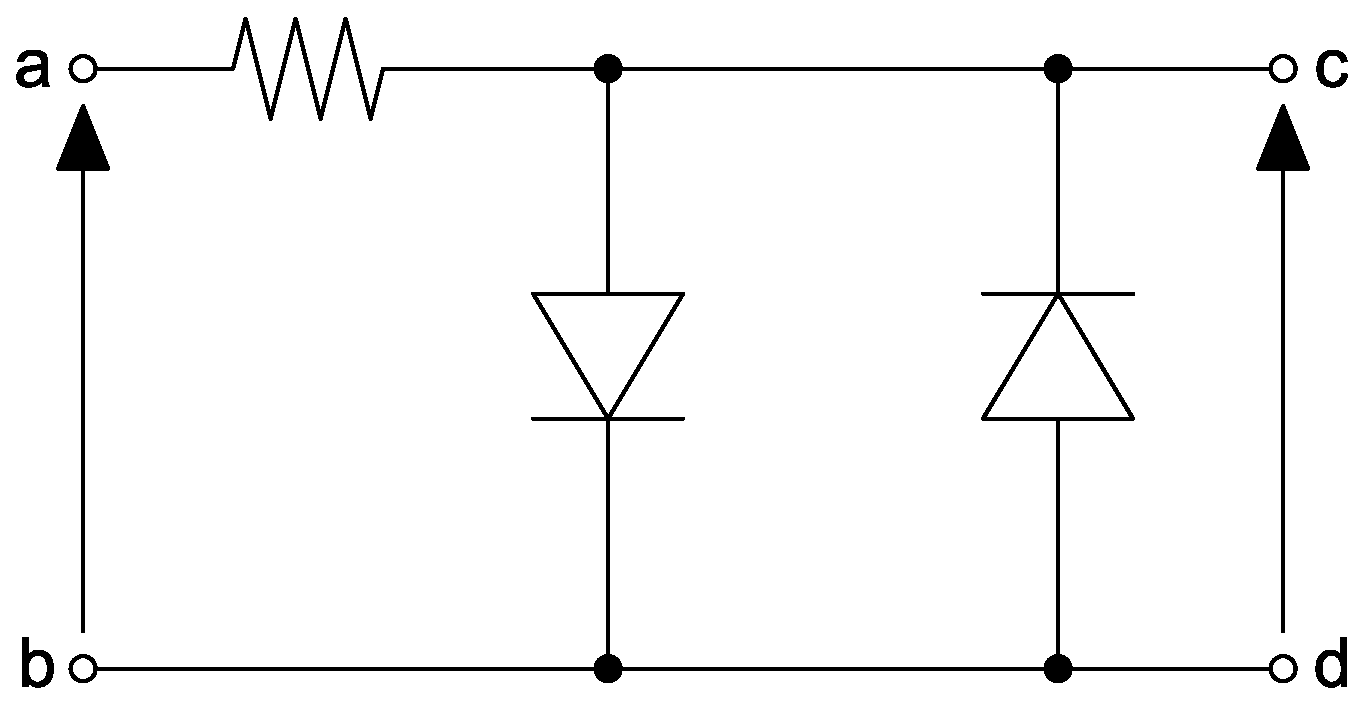
\includegraphics[width=6cm]{images/limitter.eps}
                        \caption{リミッタ回路}
                        \label{fig:limitter}
                    \end{center}
                \end{minipage}
                \begin{minipage}{0.5\hsize}
                    \begin{center}
                        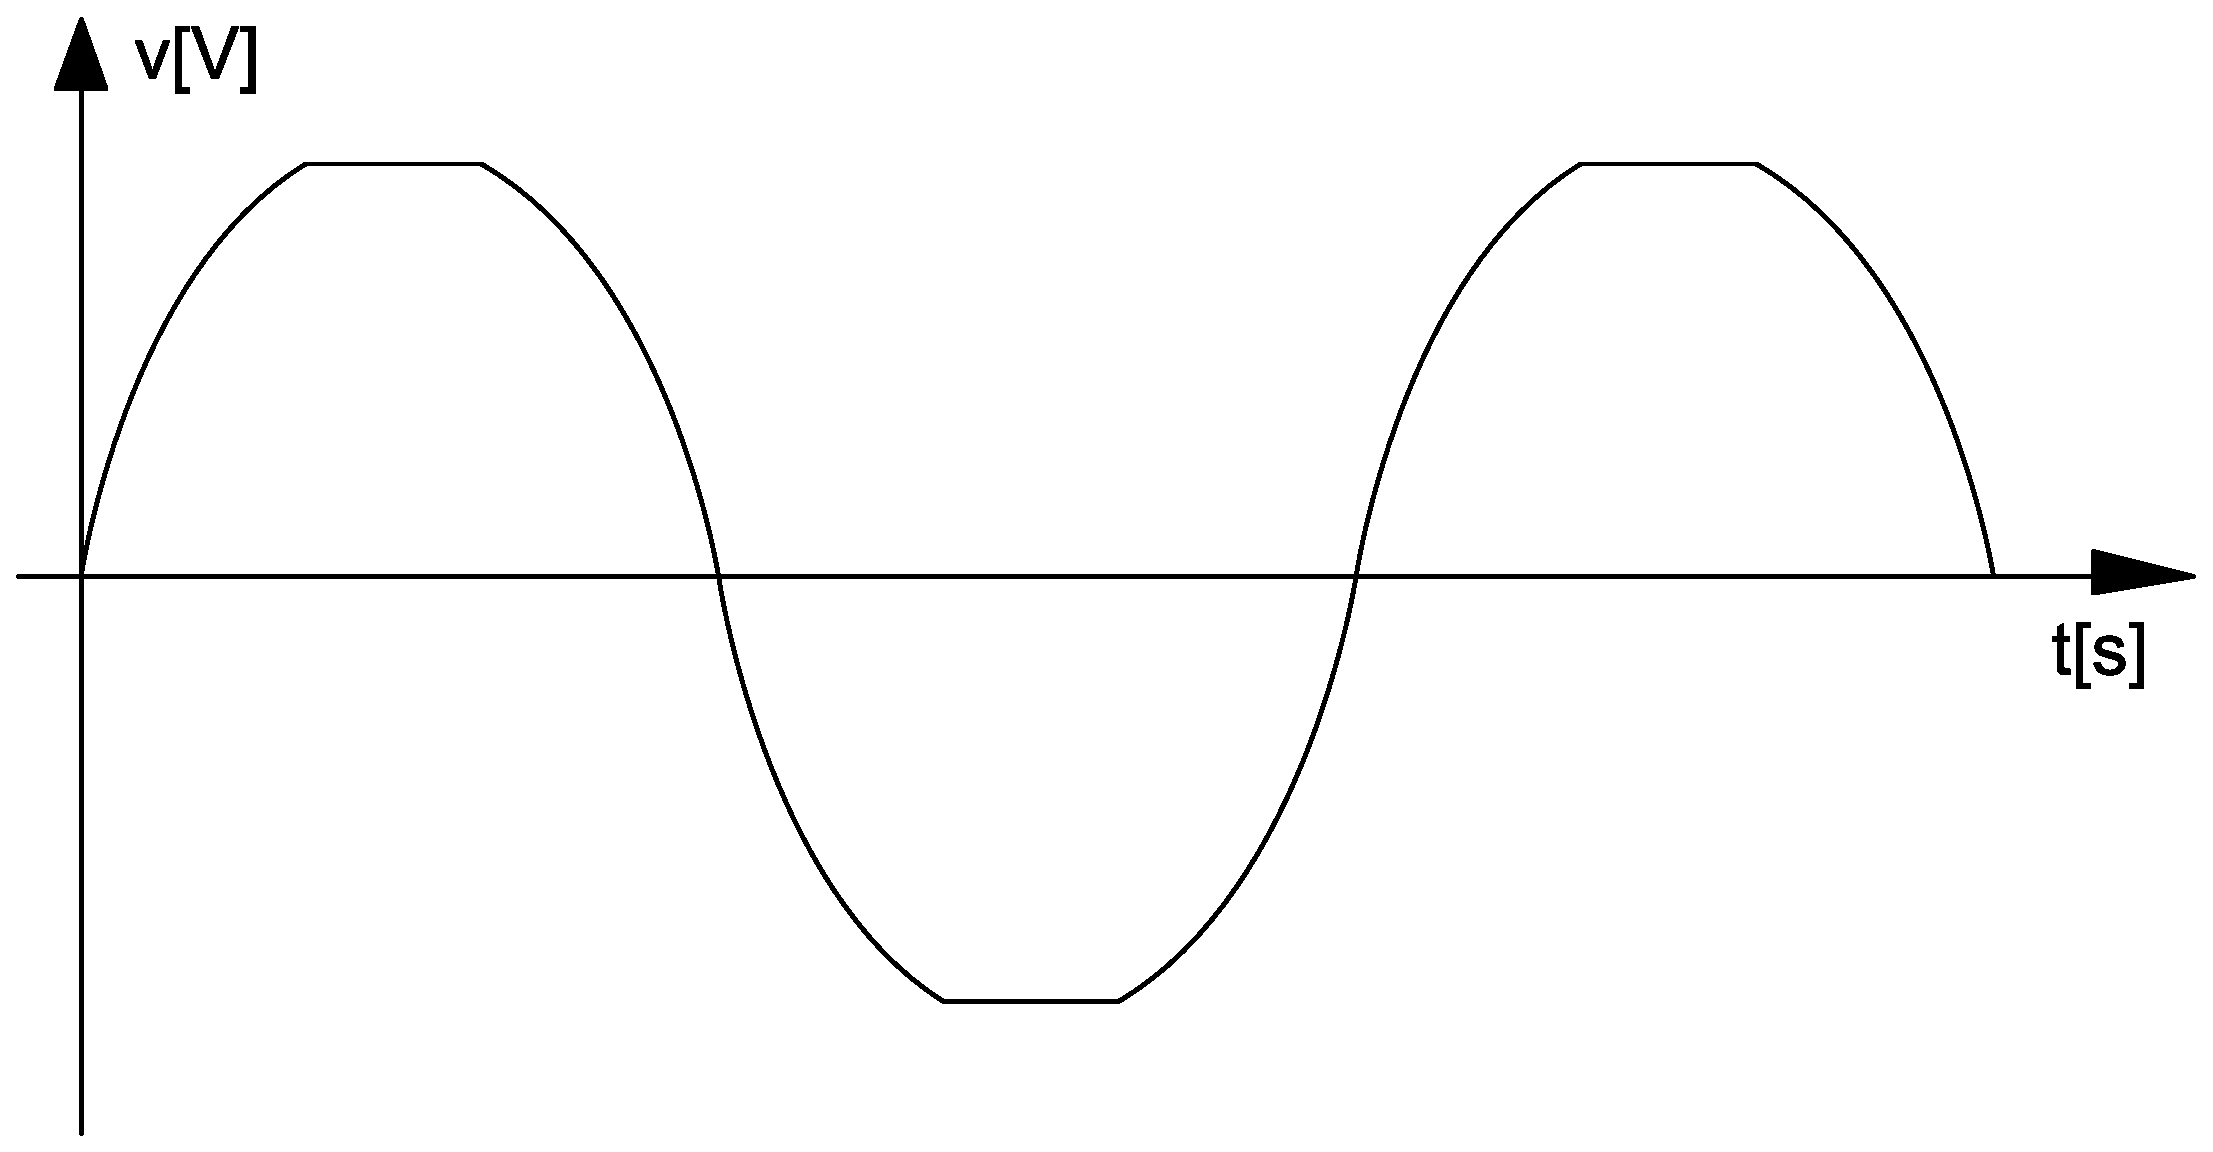
\includegraphics[width=6cm]{graphs/limitter_graph.eps}
                        \caption{リミッタ出力波形}
                        \label{fig:limitter_graph}
                    \end{center}
                \end{minipage}
            \end{figure}

    \subsection{感想}
        今回の実験では, ~ダイオードの特性を測定した.
        ~今までは電子回路などの授業中でグラフをみたことがあったが,
        ~実験を通して, ~実際に自分たちで値を測定し, ~グラフを作成することでダイオードの測定を理解することができた.

        次週はトランジスタについて測定をするので, ~予習を怠らずに臨みたい.

\section{実験B トランジスタの静特性}
    \subsection{目的}
        \begin{itemize}
            \item npn型トランジスタの静特性を測定, ~その特性を把握する.
            \item エミッタ接地回路について理解する.
        \end{itemize}

    \subsection{原理}
        npn型トランジスタは図\ref{fig:base_ground}のように二つのpn接合を背中合わせにした構造を持つ.
        ~中央のp(ベース)領域の幅は数十[$\mu$m]以下であり, ~入力側のn(エミッタ)領域の不純物濃度はベース領域よりも十分に高い.

        このようなトランジスタの入力側で, ~エミッタ側が負になるような電圧(順バイアス)$V_{EB}$を加えると,
        ~大量のエミッタ電流$I_E$が流れる. ~エミッタ電流の大部分は, ~エミッタからベースに流れ込む電子による.
        ~ベース領域の幅は十分に狭いので, ~ベースに流れ込んだ電子の大部分は再結合により失われずに
        出力側の接合(コレクタ接合)へ到達する. ~ベースに流れ込んだ電子に対し, ~コレクタへ到達する電子の割合を
        ベース接地直流電流増幅率$h_{FB}$と呼ぶ. ~コレクタ接合で,
        ~コレクタ側が正になるような電圧(逆バイアス)$V_{CB}$を加えると,
        ~コレクタ接合に到達した電子は全てコレクタに集められ, ~出力電流$I_C$となる.

        図\ref{fig:base_ground}のような回路をベース接地回路と呼ぶ.
        ~ベース接地回路では入力抵抗が低いために増幅回路としては不都合な点が多く, ~電力利得も小さいので,
        ~実際にはエミッタ接地回路で使われることが多い.

    \subsection{実験方法}
        \subsubsection{注意点}
            \begin{itemize}
                \item 電源のスイッチをONにする前に, ~回路の接続と計測機器の設定を十分に確認する.
                \item 各実験について, ~電圧や電流の範囲が指定された値を超えないよう,
                    ~注意しながら実験を進める.
                \item 電圧や電流の測定値は表にまとめ, ~電圧-電流の関係をグラフにまとめる.
            \end{itemize}

        図\ref{fig:emitter_ground}のようなエミッタ接地回路の接続を行う.

        \begin{figure}[ht]
            \begin{minipage}{0.5\hsize}
                \begin{center}
                    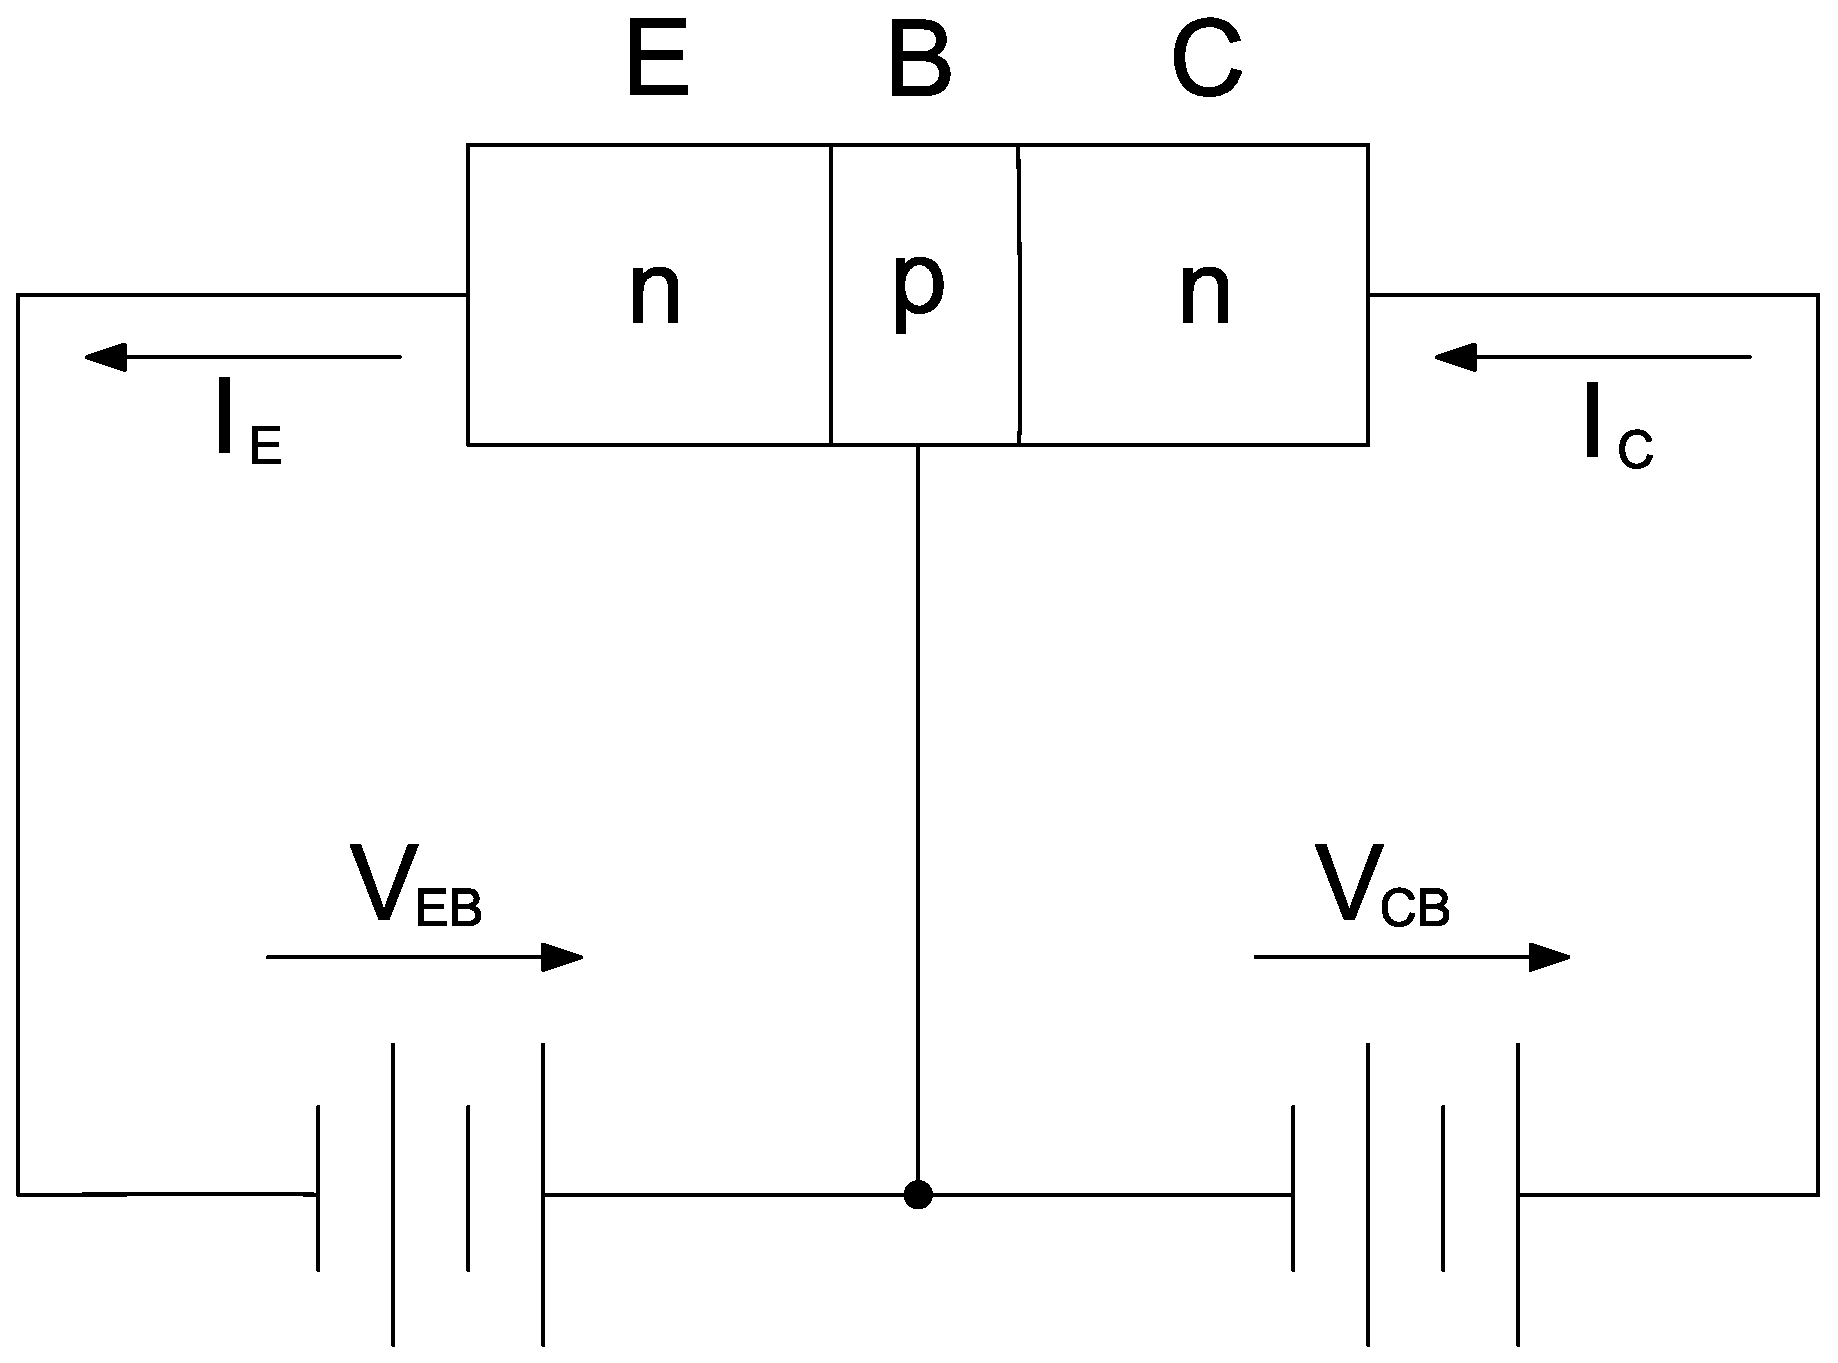
\includegraphics[width=6cm]{images/base_ground.eps}
                    \caption{ベース接地回路}
                    \label{fig:base_ground}
                \end{center}
            \end{minipage}
            \begin{minipage}{0.5\hsize}
                \begin{center}
                    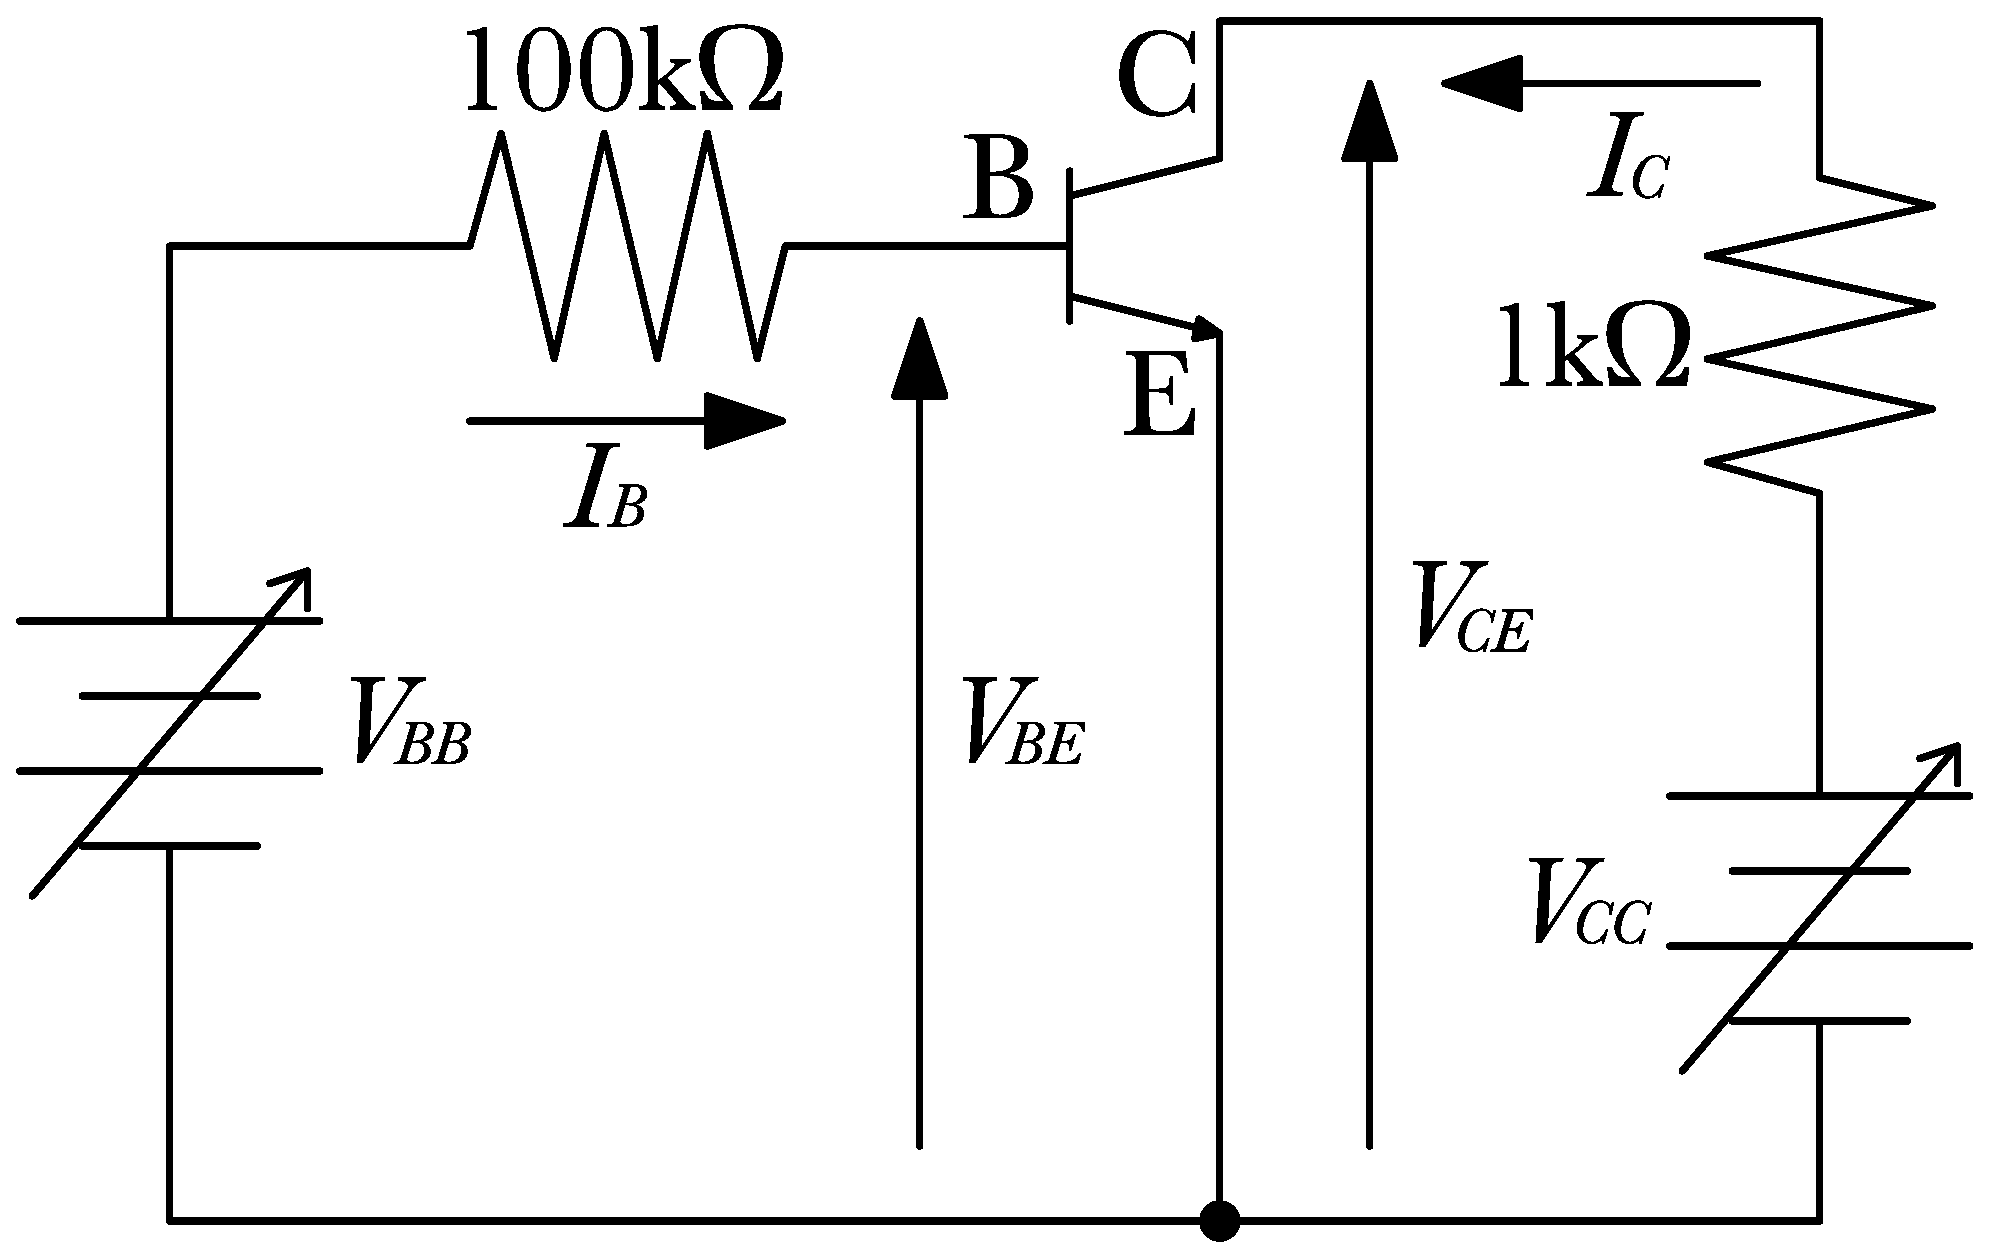
\includegraphics[width=6cm]{images/emitter_ground.eps}
                    \caption{エミッタ接地回路}
                    \label{fig:emitter_ground}
                \end{center}
            \end{minipage}
        \end{figure}

        \subsubsection{$V_{BE}$-$I_B$特性の測定}
            $V_{CE}$を0.5, 1.5, 2.5[V]と定め, ~$I_B$が0〜15[$\mu$A]の範囲での$V_{BE}$, $I_C$を測定する.
            ~$I_B$, $I_C$は抵抗の端子間電圧を測定して算出する.

        \subsubsection{$V_{CE}$-$I_C$特性の測定}
            $I_B$を2, 4, 6, 8, 10[$\mu$A]と定め, ~$V_{CE}$が0〜10[V]の範囲での$I_C$を測定する.

    \subsection{使用器具}
        \begin{description}
            \item[トランジスタ] EC-02
            \item[デジタルマルチメーター] Ec-03, Ec-14
            \item[交流電源] Ec-07, Ec-11
        \end{description}

    \subsection{実験結果}
        \subsubsection{$V_{BE}$-$I_B$特性の測定}
            $V_{BE}$-$I_B$特性グラフ, ~$I_B$-$I_C$特性グラフ, ~測定値の表を以下に示す.

            \begin{figure}[ht]
                \begin{minipage}{0.5\hsize}
                    \begin{center}
                        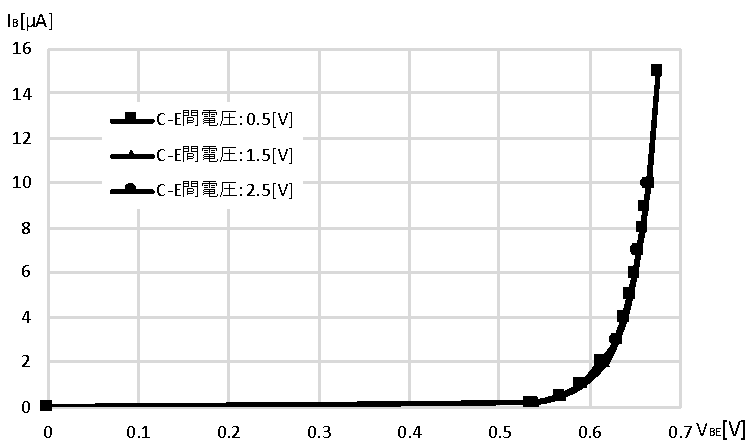
\includegraphics[width=8cm]{graphs/VBE-IB_graph.pdf}
                        \caption{$V_{BE}$-$I_B$特性グラフ}
                        \label{fig:VBE-IB_graph}
                    \end{center}
                \end{minipage}
                \begin{minipage}{0.5\hsize}
                    \begin{center}
                        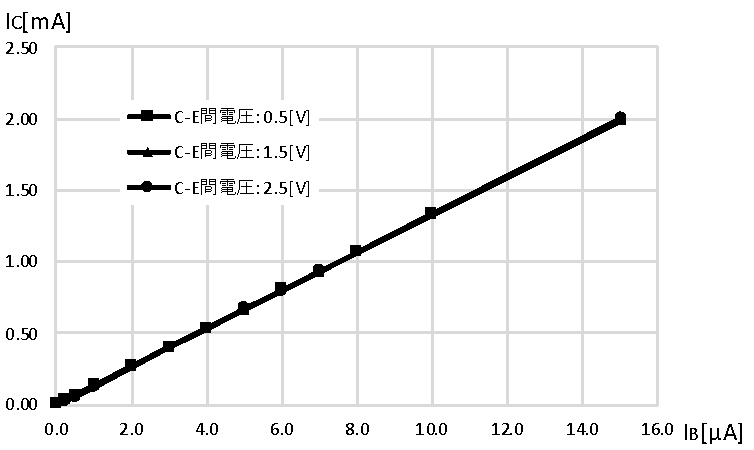
\includegraphics[width=8cm]{graphs/IB-IC_graph.pdf}
                        \caption{$I_B$-$I_C$特性グラフ}
                        \label{fig:IB-IC_graph}
                    \end{center}
                \end{minipage}
            \end{figure}

            \begin{table}[ht]
                \begin{center}
                    \caption{$V_{BE}$-$I_B$特性測定値}
                    \label{tab:VBE-IB}
                    \begin{tabular}{c||c|c||c|c||c|c}
                        $V_{CE}$[V] & \multicolumn{2}{c||}{0.5} & \multicolumn{2}{c||}{1.5} & \multicolumn{2}{c}{2.5} \\ \hline
                        $I_B$[$\mu$A] & $V_{BE}$[V] & $I_C$[mA] & $V_{BE}$[V] & $I_C$[mA] & $V_{BE}$[V] & $I_C$[mA] \\ \hline \hline
                        0.0 & 0.00 & 0.00 & 0.00 & 0.00 & 0.00 & 0.00 \\
                        0.2 & 0.54 & 0.03 & 0.54 & 0.03 & 0.54 & 0.02 \\
                        0.5 & 0.57 & 0.06 & 0.57 & 0.07 & 0.57 & 0.05 \\
                        1.0 & 0.59 & 0.13 & 0.59 & 0.13 & 0.59 & 0.12 \\
                        2.0 & 0.61 & 0.26 & 0.62 & 0.27 & 0.62 & 0.26 \\
                        3.0 & 0.63 & 0.40 & 0.63 & 0.40 & 0.63 & 0.40 \\
                        4.0 & 0.64 & 0.53 & 0.64 & 0.53 & 0.64 & 0.53 \\
                        5.0 & 0.65 & 0.66 & 0.64 & 0.67 & 0.65 & 0.67 \\
                        6.0 & 0.65 & 0.80 & 0.65 & 0.80 & 0.65 & 0.80 \\
                        7.0 & 0.66 & 0.93 &  &  & 0.65 & 0.93 \\
                        8.0 & 0.66 & 1.06 & 0.66 & 1.07 &  &  \\
                        10.0 & 0.67 & 1.33 & 0.67 & 1.34 & 0.66 & 1.33 \\
                        15.0 & 0.68 & 1.99 & 0.68 & 2.01 & 0.68 & 2.00
                    \end{tabular}
                \end{center}

            \end{table}

            $V_{BE}$-$I_B$特性のグラフを見ると, ~$V_{CE}$が変化しても, ~測定値にほとんど変化がないことがわかる.
            ~実験Aのダイオードの順方向特性と同じように, ~$V_{BE}$が0.55[V]を超えたあたりで急激に電流が流れ出している.

            また, ~$I_B$-$I_C$特性グラフをみると, ~美しい比例関係にあることがわかる.
            ~こちらも, ~$V_{BE}$-$I_B$特性と同じく, ~$V_{CE}$が変化しても測定値に変化は見られない.

            ここで, ~直流電流増幅率$h_{FE}$, ~小信号電流増幅率$h_{fe}$を以下のように定義する.

            \begin{eqnarray*}
                h_{FE} &=& \frac{I_C}{I_B} \\
                h_{fe} &=& \frac{\Delta I_C}{\Delta I_B}
            \end{eqnarray*}

            直流電流増幅率は, ~コレクタ電流とベース電流の比で, ~$I_B$-$I_C$特性グラフ.
            ~この値が大きいほど, ~その回路が入力電流を大きく増幅する.

            一方小信号電流増幅率は, グラフの局所的な傾きで, ~特定の電流値での増幅率を表す.

        \subsubsection{$V_{CE}$-$I_C$特性の測定}
            図\ref{fig:VCE-IC_graph}, 表\ref{tab:VCE-IC}に$V_{CE}$-$I_C$特性グラフと測定値の表を示す.

            \begin{figure}[ht]
                \begin{center}
                    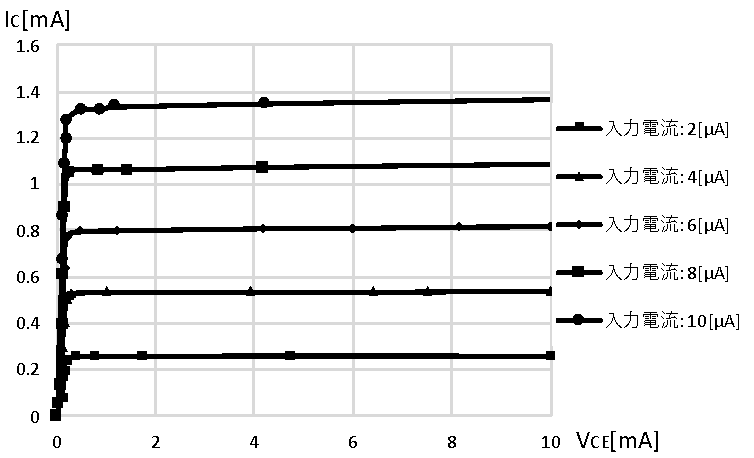
\includegraphics[width=12cm]{graphs/VCE-IC_graph.pdf}
                    \caption{$V_{CE}$-$I_C$特性グラフ}
                    \label{fig:VCE-IC_graph}
                \end{center}
            \end{figure}
            \begin{table}[ht]
                \begin{center}
                    \caption{$V_{CE}$-$I_C$特性測定値}
                    \label{tab:VCE-IC}
                    \renewcommand{\arraystretch}{0.8}
                    \begin{tabular}[t]{c|c||c|c||c|c||c|c||c|c}
                        \multicolumn{2}{c||}{$I_B$[$\mu$A] \qquad 2.0 \qquad} & \multicolumn{2}{c||}{4.0} &
                            \multicolumn{2}{c||}{6.0} & \multicolumn{2}{c||}{8.0} & \multicolumn{2}{c}{10} \\ \hline
                         $V_{CE}$[V] & $I_C$[mA] & $V_{CE}$[V] & $I_C$[mA] & $V_{CE}$[V]
                            & $I_C$[mA] & $V_{CE}$[V] & $I_C$[mA] & $V_{CE}$[V] & $I_C$[mA] \\ \hline \hline
                         0.00 & 0.00 & 0.00 & 0.00 & 0.00 & 0.00 & 0.00 & 0.00 & 0.00 & 0.00 \\
                         0.11 & 0.09 & 0.09 & 0.10 & 0.08 & 0.12 & 0.05 & 0.05 & 0.13 & 0.68 \\
                         0.13 & 0.17 & 0.13 & 0.30 & 0.12 & 0.38 & 0.07 & 0.13 & 0.14 & 0.86 \\
                         0.17 & 0.20 & 0.15 & 0.40 & 0.16 & 0.64 & 0.11 & 0.39 & 0.16 & 1.09 \\
                         0.19 & 0.24 & 0.20 & 0.50 & 0.21 & 0.77 & 0.13 & 0.61 & 0.19 & 1.19 \\
                         0.37 & 0.26 & 0.23 & 0.52 & 0.46 & 0.80 & 0.17 & 0.90 & 0.21 & 1.28 \\
                         0.74 & 0.26 & 0.27 & 0.53 & 1.20 & 0.80 & 0.26 & 1.05 & 0.51 & 1.32 \\
                          &  & 1.00 & 0.54 &  &  & 0.84 & 1.06 & 0.86 & 1.32 \\
                         1.74 & 0.26 &  &  &  &  & 1.44 & 1.06 & 1.17 & 1.33 \\
                         4.71 & 0.26 & 3.90 & 0.54 & 4.19 & 0.81 & 4.17 & 1.07 & 4.20 & 1.35 \\
                          &  & 6.39 & 0.54 & 6.00 & 0.81 &  &  &  &  \\
                          &  & 7.49 & 0.54 & 8.13 & 0.82 &  &  &  &  \\
                         10.00 & 0.26 & 10.00 & 0.54 & 9.98 & 0.82 & 10.00 & 1.09 & 10.00 & 1.37
                     \end{tabular}
                \end{center}
            \end{table}

            グラフを見ると, ~$V_{CE}$をかけると急激に$I_C$が流れ出すことがわかる.
            ~流れ始めた$I_C$は, ~$V_{CE}$が約0.2[V]に達した時点で頭打ちとなり,
            ~その後はほとんど増えない.

            また, ~$I_B$が増えると$I_C$の上限値が増え, ~グラフの線が縦軸方向に伸びていることがわかる.

            結果から, $V_{CE} = 6$[V], $I_B = 6$[$\mu$A]での$h_{FE}$, $h_{fe}$を求めてみる.

            ~表\ref{tab:VCE-IC}より$h_{FE}$を求めると,

            \[
                h_{FE} = \frac{I_C}{I_B} = \frac{0.81 \times 10^{-3}}{6.0 \times 10^{-6}} = 135
            \]

            $V_{CE}$の値によって$h_{fe}$の値がほとんど変わらないことは$V_{BE}$-$I_B$特性の測定でわかったので,
            図\ref{fig:IB-IC_graph}から$I_C$が5〜7[V]の範囲で$h_{fe}$を求めてみると,

            \[
                h_{fe} = \frac{\Delta I_C}{\Delta I_B} = \frac{(0.93 - 0.66) \times 10^{-3}}{(7.0 - 5.0) \times 10^{-6}} = 135
            \]

            今回の実験では, ~$h_{FE} = h_{fe}$となった.

    \subsection{感想}
        $V_{BE}$-$I_B$特性を測定し, ~ダイオードの順方向特性と同じことがわかった.
        ~これらはどちらも一つのpn接合部分での特性なので今までは机上で同じであろうと考えることはできたが,
        ~今回の二つの実験を通して改めて体感, ~考察することができた.

        ~また, ~教科書に載っている各特性のグラフでは, ~$V_{BE}$-$I_B$特性と$I_B$-$I_C$特性が固定の$V_{CE}$の時しか
        示されておらず, ~実験を通して, ~$V_{CE}$が変化しても変わらないことが確かめられ, ~理解が深まった.

\begin{thebibliography}{99}
    \bibitem{} 木村圭一郎ほか, ~『電子回路』, ~コロナ社
\end{thebibliography}
\end{document}
